%========================================
% Beamer "Singapore" Theme Template
%========================================
\documentclass[aspectratio=169]{beamer}

% THEME
\usetheme{Singapore}

% COLORS & FONTS
\definecolor{brand}{RGB}{45,110,191}
\definecolor{accent}{RGB}{5,155,192}
\definecolor{hrgray}{RGB}{100,100,100}
\setbeamercolor{structure}{fg=brand}
\setbeamercolor{title}{fg=hrgray}
\setbeamercolor{subtitle}{fg=brand}
\setbeamercolor{author}{fg=hrgray}
\setbeamercolor{date}{fg=hrgray}
\setbeamercolor{frametitle}{fg=hrgray}
\setbeamercolor{block title}{fg=white,bg=brand}
\setbeamercolor{block body}{bg=black!2}
\usepackage{lmodern}
\usefonttheme{professionalfonts}

\usepackage{comment}
\usepackage{etoolbox}
\usepackage[T1]{fontenc}
\usepackage[utf8]{inputenc}
\usepackage{microtype}
\usepackage{graphicx}
\usepackage{tikz}
\usepackage{xcolor}

\setbeamertemplate{navigation symbols}{}

\setbeamertemplate{footline}{
  \leavevmode
  \hbox{
    \begin{beamercolorbox}[wd=.5\paperwidth,ht=3ex,dp=1ex,left]{author in head/foot}
      \hspace{0.8ex}{
\includegraphics[height=0.7cm]{img/logo.png}}
    \end{beamercolorbox}%
    \begin{beamercolorbox}[wd=.5\paperwidth,ht=3ex,dp=1ex,right]{date in head/foot}
      \insertframenumber{} / \inserttotalframenumber\hspace{2ex}
    \end{beamercolorbox}%
  }
  \vskip0pt
}

% METADATA
\title[Short Title]{\bfseries{Basic Chatbot Guidance}}
\subtitle{Discussion Starter}
\author[Patrick Hall]{\textbf{Patrick Hall}}
\institute{HallResearch.ai}
\date{\today}

% handle URLs/links
\PassOptionsToPackage{hyphens}{url}\usepackage{hyperref}
\urlstyle{same}
\hypersetup{
    colorlinks=true,
    urlcolor=[rgb]{0.0196, 0.6078, 0.7529},
    linkcolor=[rgb]{0.17647, 0.388, 0.749},
    citecolor=[rgb]{0.0196, 0.6078, 0.7529}
}

% Chicago citations and bibliography
\setbeamertemplate{bibliography item}[text]
\usepackage[authordate]{biblatex-chicago}
\setbeamertemplate{frametitle continuation}{}
\addbibresource{references.bib}
\setlength{\bibitemsep}{0.5\baselineskip}
\AtBeginBibliography{\scriptsize}
\renewcommand\UrlFont{\sffamily}

\begin{document}

%-------------------------
\begin{frame}

  \titlepage
  \begin{tikzpicture}[remember picture,overlay]
    \node[opacity=0.1] at (current page.center)
      {
\includegraphics[width=0.55\paperwidth]{img/hrwater.png}};
  \end{tikzpicture}
  \centering\scriptsize{\color{hrgray}{\textcopyright~2026 Patrick Hall (ph@hallresearch.ai). Some rights reserved.\\Text and copy are licensed under a Creative Commons Attribution-NonCommercial-ShareAlike 4.0 International License (CC BY-NC-SA 4.0).}}

\end{frame}

%-------------------------
\begin{frame}{Agenda}\small
  \tableofcontents
  \vspace{10pt}
  \textbf{Optional Prerequisites:} Access to Gemini \href{https://tinyurl.com/3zvh5b47}{chatbot} through NIST, an \href{https://www.overleaf.com/}{Overleaf} account or your favorite LaTeX editor.  
  
\end{frame}

%------------------------------------------------
\section{Good Practices}

%------------------------------------------------
\begin{frame}[t]{Chatbots—Good Practices}
\small
\setlength{\leftmargini}{1.2em}
\setlength{\leftmarginii}{1.1em}

\begin{columns}[T,onlytextwidth]
    \column{0.48\textwidth}
    \textbf{Good Practices:}
    \begin{itemize}
        \setlength\itemsep{0.15em}
        \setlength\parskip{0pt}
        \setlength\parsep{0pt}
        \item Anonymize sensitive inputs.
        \item Disclose chatbot use when required.
        \begin{itemize}
            \setlength\itemsep{0.05em}
            \setlength\parskip{0pt}
            \setlength\parsep{0pt}
            \item Follow applicable policy.
            \item Especially with consequential uses.
        \end{itemize}
        \item Break down large tasks; \href{https://github.com/hallresearch-ai/basic-chatbot-guidance/blob/main/prompt-library/ai-guidance-proof.txt}{clearly mark long instructions}.
        \item Use rubrics with calibration.
        \item Provide examples and grounding data.
        \item Ask for options, alternatives, critiques, and feedback.
    \end{itemize}

    \column{0.48\textwidth}
    \textbf{Basic Tools:}
    \begin{itemize}
        \setlength\itemsep{0.15em}
        \setlength\parskip{0pt}
        \setlength\parsep{0pt}
        \item Draft prompts in a text editor or word processor.
        \item Maintain a \href{https://github.com/hallresearch-ai/basic-chatbot-guidance/tree/main/prompt-library}{prompt library}.
        \begin{itemize}
            \setlength\itemsep{0.05em}
            \setlength\parskip{0pt}
            \setlength\parsep{0pt}
            \item Text files, GitHub, or open-source packages.
            \item \href{https://github.com/hallresearch-ai/basic-chatbot-guidance/blob/main/prompt-library/natural-style-guide.txt}{Personal style guides}.
            \item \href{https://github.com/hallresearch-ai/basic-chatbot-guidance/blob/main/prompt-library/short-doc-proof.txt}{Verification prompts}.
        \end{itemize}
    \end{itemize}
\end{columns}
\end{frame}


%------------------------------------------------
\section{Common Pitfalls}

%------------------------------------------------
\begin{frame}{Chatbots—When to Use Other Tools}
\textbf{Understand when to use other types of AI:}\small
\vspace{-1em}
\begin{columns}
    \column{0.55\textwidth}
    \vspace{1em}
    \begin{itemize}
        \item Optimization, statistics, and ML for rigorous data analysis.
        \item Real-time/real-world sensor systems for live information (traffic, weather, etc.).
        \item Qualitative methods for developing bibliographies or ``ground truth'' information. 
            \begin{itemize}
                \item Use more credible search or research tools to find or confirm sources of record.
            \end{itemize}
    \end{itemize}

    \column{0.45\textwidth}
    \centering
    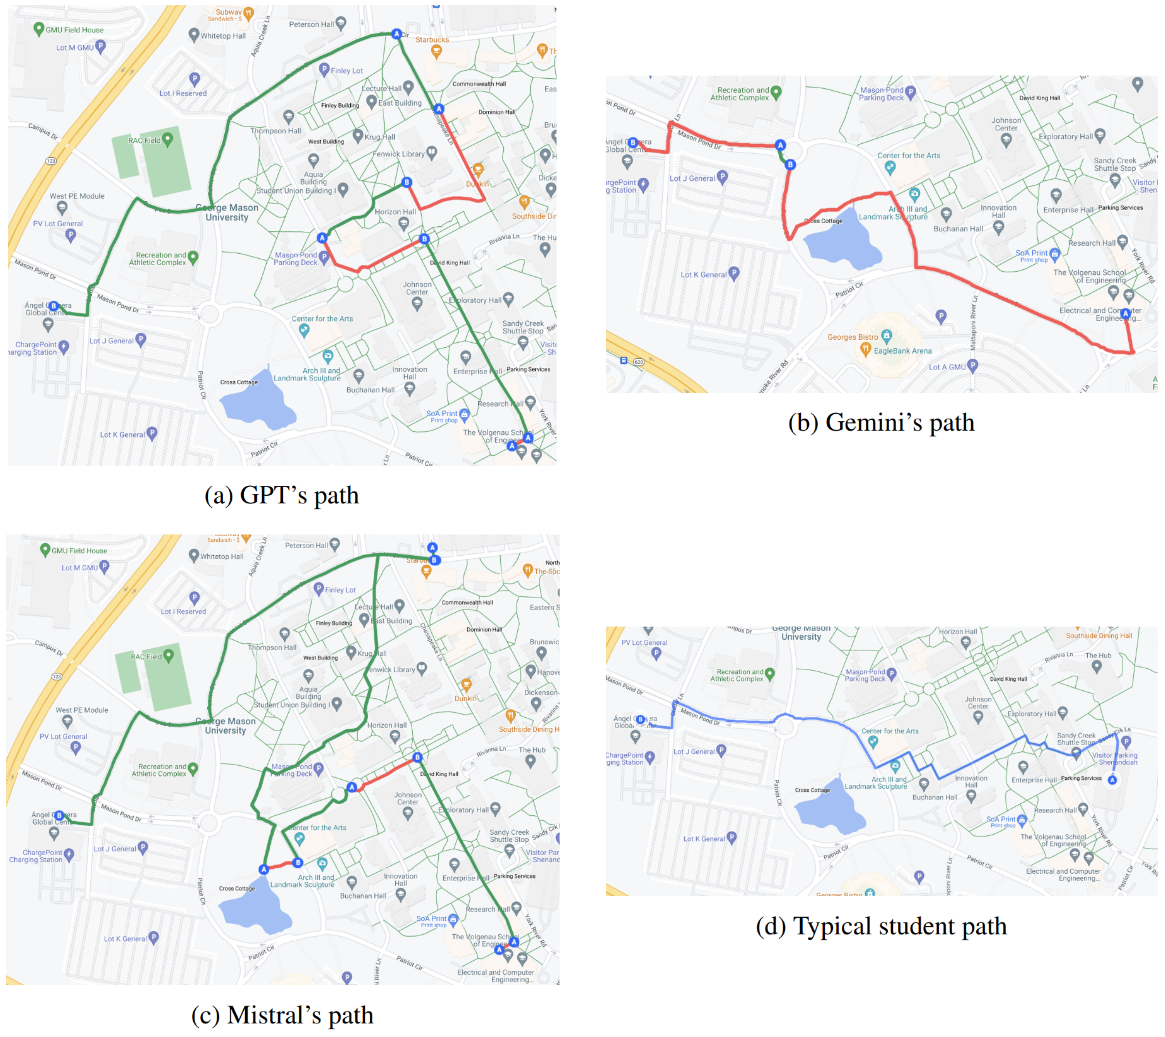
\includegraphics[width=0.8\linewidth]{img/bad_map.png}\\
    \scriptsize Illogical mapping decisions from language models on GMU campus \parencite{chen2024can}.
\end{columns}
\end{frame}

%------------------------------------------------
\begin{frame}[t]{Chatbots—Common AI Fails\\
\small{\parencite{TowardsaStandardforI537, ArtificialIntelligen058}}}
\begin{columns}[T]
    \column{0.5\textwidth}
    \textbf{How AI Fails You:}
    \vspace{0.8em}
    \begin{itemize}
        \item Hallucinating or fabricating information.
        \item Generating fake citations.
        \item Combining true information incorrectly.
        \item Poor knowledge of the physical world.
        \item Failing at complex reasoning tasks.
        \item Misusing or exposing sensitive information.
    \end{itemize}

    \column{0.5\textwidth}
    \textbf{How You Fail with AI:}
    \vspace{0.8em}
    \begin{itemize}
        \item Allowing outputs to confirm pre-existing biases.
        \item Anthropomorphizing AI (AI does not ``think,'' ``understand,'' ``feel''), including emotional entanglement.
        \item Anchoring to AI outputs as first-seen information.
        \item Accepting sycophantic responses.
        \item Inputting sensitive information.
    \end{itemize}
\end{columns}
\end{frame}

%------------------------------------------------
\section{What Usually Works Well}

%------------------------------------------------
\begin{frame}[t]{Chatbots—What Usually Works Well}
\normalsize
\begin{columns}

    \column{0.58\textwidth}
    \begin{itemize}
        \item Text-centered tasks:
        \begin{itemize}
            \item Drafting, ideally from an outline.
            \item Summarizing.
            \item Polishing and editing.
            \item Identifying themes.
        \end{itemize}
        \item Generating structured outputs: HTML, LaTeX, spreadsheets.
        \item Initial research and source discovery.\\
    \end{itemize}
    \vspace{1em}
    {\scriptsize Always consider human-AI teaming, e.g., supplementing decision-making with statistical models, or as discussed in \cite{HumanAITeamingStateo282}.}

    \column{0.42\textwidth}
    \centering
    
\includegraphics[width=0.8\linewidth]{img/bad_search.jpg}\\
    \scriptsize A well-known Google AI search failure.
    
\end{columns}
\end{frame}

%------------------------------------------------
\section{Basic Writing Workflows}

\begin{frame}[t]{Chatbots—Writing Workflows}
\textbf{Don’t let chatbots write for you end-to-end} \parencite{alkaissi2023artificial}.

\vspace{1em}

\textbf{Recommended workflow:}
\begin{itemize}
    \item You create the outline.
    \begin{itemize}
        \item You add citations, figures, tables, and validation.
    \end{itemize}
    \item Chatbots draft the outline into coherent text.
    \item You proofread and edit.\\
\end{itemize}
\vspace{5pt}
OR\\ 
\vspace{10pt}
Ask chatbots for feedback, critique, and editing help. Use tools like Grammarly for more thorough copy-editing.\\ 
\vspace{1em}
\textbf{Writing mini-exercise ...} 
\end{frame}

%------------------------------------------------
\begin{frame}{Chatbots—Writing Mini-exercise}

\footnotesize
\textbf{Example materials:} \href{https://github.com/hallresearch-ai/basic-chatbot-guidance/tree/main/model-doc-outline}{hallresearch-ai/basic-chatbot-guidance}. \\
\vspace{1em} 
Start with a polite salutation and orient the chatbot to the writing exercise at hand: ``\texttt{Hi, I need help converting outline bullets into a paragraph of text for a blog post about X.}''\\
\vspace{1em}
Gather references, create tables and figures, and compose materials into an outline. Ask the chatbot to draft your bullets into paragraphs, referencing the provided tables, figures, and citations, and if necessary, to avoid creating any new tables, figures, and citations. \\
\vspace{1em}
If using a technical format, e.g., LaTeX or AsciiDoc, have the chatbot generate this format directly.\\
\vspace{1em}
OR\\
\vspace{1em}
Ask a chatbot to edit or provide feedback on something you have drafted. Ask for help with flow, concision, clarity, transitions, appropriateness for audience, omissions, etc.\\

\end{frame}

%------------------------------------------------

\section*{}
{
\setbeamertemplate{headline}{}
\begin{frame}[t, allowframebreaks]{References}
  \printbibliography[heading=none]
\end{frame}
}

\end{document}